\documentclass[11pt,a4paper]{article}
\usepackage[margin=0.75in]{geometry}
\usepackage{lmodern}
\usepackage[T1]{fontenc}
\usepackage{amsmath,amssymb,amsfonts}
\usepackage{graphicx}
\usepackage{booktabs}
\usepackage{xcolor}
\usepackage{hyperref}
\usepackage{caption}
\usepackage{subcaption}
\usepackage{float}
\usepackage{enumitem}
\usepackage{fancyhdr}

\hypersetup{
    colorlinks=true,
    linkcolor=blue!70!black,
    citecolor=blue!70!black,
    urlcolor=blue!70!black
}

\pagestyle{fancy}
\fancyhf{}
\rhead{\small \textit{Project 2: Medical AI Reliability \& Selective Prediction}}
\lhead{\small \textit{Research Report}}
\cfoot{\thepage}

\title{\textbf{\Large AI That Knows When a Medical Image Cannot Be Trusted:\\
Selective Prediction, Epistemic Uncertainty Quantification, and Out-of-Distribution Screening for Safe Clinical Deployment}}
\author{\textbf{Research Portfolio Project 2} \\
\normalsize Colorectal Histopathology Reliability Benchmark (PathMNIST, DermaMNIST, BloodMNIST)}
\date{\normalsize October 2026}

\begin{document}

\maketitle

\begin{abstract}
\noindent Modern deep learning classifiers for medical imaging regularly demonstrate high headline accuracy on standard benchmarks, yet they remain dangerously susceptible to catastrophic overconfidence. When presented with physical image corruptions (stage vibration, optical defocus, detector noise, or chemical stain fading) or foreign clinical domains, standard architectures routinely assert incorrect diagnoses with deceptively high confidence ($>90\%$). In high-stakes clinical settings, such ``silent failures'' jeopardize patient safety. In this work, we design, implement, and systematically audit \textbf{AI That Knows When a Medical Image Cannot Be Trusted}---a multi-signal safety triage framework that couples deep residual classification with deterministic image quality assessment (IQA), inference-time Monte Carlo Dropout for epistemic uncertainty quantification, validation-fitted temperature calibration, and deep feature Out-of-Distribution (OOD) screening. Benchmarked on the PathMNIST benchmark (107,180 images, colorectal histopathology, CC BY 4.0), our classifier achieves 86.07\% diagnostic accuracy on a held-out locked test partition (7,180 images). Post-hoc temperature scaling ($T=1.23$) reduces Expected Calibration Error (ECE) from 6.56\% to 5.17\% (a 21.2\% reduction in overconfidence). Epistemic uncertainty demonstrates strong error-predictive ability (Error Detection AUROC = 0.7908; Area Under Risk-Coverage curve $\text{AURC} = 4.80$). Crucially, our failure analysis reveals that 29.2\% of model errors on clean images are ``silent failures'' (high confidence, low entropy), demonstrating that uncertainty alone is insufficient. Under controlled stress testing, deep feature Mahalanobis distance achieves 98.9\%--99.3\% OOD AUROC ($\text{FPR}_{95} \le 1.0\%$) on foreign clinical domains (DermaMNIST, BloodMNIST), whereas standard softmax and energy metrics fail (AUROC 42\%--57\%). Furthermore, under severe optical defocus blur, the selective triage policy achieves a 100\% automated clinical deferral rate. These results establish that safe clinical AI requires a multi-layered defense-in-depth architecture combining physical, representational, and uncertainty-aware signals.
\end{abstract}

\vspace{0.5em}

%%%%%%%%%%%%%%%%%%%%%%%%%%%%%%%%%%%%%%%%%%%%%%%%%%%%%%%%%%%%%%%%%%%%%%%%%%%%%%%
\section{INTRODUCTION}
%%%%%%%%%%%%%%%%%%%%%%%%%%%%%%%%%%%%%%%%%%%%%%%%%%%%%%%%%%%%%%%%%%%%%%%%%%%%%%%
The rapid translation of computer vision into diagnostic medicine holds immense potential for alleviating global pathologist workloads, standardizing cancer screening, and reducing diagnostic turnaround times. In computational pathology, convolutional neural networks routinely report diagnostic accuracy rivaling experienced clinicians on curated benchmark datasets. 

However, a fundamental disconnect persists between controlled benchmark performance and clinical deployment safety. Standard deep neural networks are closed-world discriminative models: forced to map any input $x$ to a fixed probability simplex $\sum_{c=1}^C p_c = 1$, they are mathematically incapable of declaring \textit{``I do not know''}. When exposed to real-world acquisition degradations---such as microscope stage motor vibration, focal plane defocus, photon-starved detector noise, or reagent batch variation in Hematoxylin and Eosin (H\&E) staining---these models do not gracefully degrade. Instead, they produce confidently wrong predictions. Worse, when an image from a completely different clinical modality is inadvertently routed to the model, standard softmax outputs frequently assign high probabilities to arbitrary target classes.

In clinical decision support, a false positive or missed malignant diagnosis delivered with $>95\%$ artificial confidence is far more hazardous than a system that explicitly defers ambiguous scans. The primary objective of this project is to build an AI system that not only predicts tissue histology, but possesses \textbf{meta-cognitive awareness}: the capability to detect when an image is physically corrupted, out-of-distribution, or when its internal prediction is unreliable, automatically flagging the scan and abstaining from autonomous diagnosis in favor of expert human review.

\noindent\textbf{Key Contributions of this Project:}
\begin{enumerate}[leftmargin=*]
    \item \textbf{Defense-in-Depth Architecture:} We formulate a multi-signal triage policy combining deterministic physical Image Quality Assessment (IQA), latent feature Out-of-Distribution (OOD) distance, Monte Carlo Dropout epistemic uncertainty, and post-hoc calibrated confidence.
    \item \textbf{Strict Partition Hygiene:} All calibration parameters ($T$) and operational abstention thresholds ($\tau$) are fitted strictly on the validation set, ensuring evaluation on the held-out test partition (7,180 images) remains untouched.
    \item \textbf{Discovery of Silent Failures:} We empirically quantify that 29.2\% of model errors on clean test images occur with high confidence ($>85\%$) and low entropy ($<0.35$), providing direct experimental proof that epistemic uncertainty alone is insufficient for clinical safety.
    \item \textbf{Superiority of Latent Manifold OOD Detection:} We demonstrate that deep feature Mahalanobis distance achieves $>98.9\%$ AUROC with $\le 1.0\%$ false positive rate against near-medical OOD domains (DermaMNIST and BloodMNIST), whereas baseline Maximum Softmax Probability (MSP) and Free Energy scoring collapse to random performance (42\%--57\%).
    \item \textbf{Reproducible Open-Source Pipeline \& Interactive Dashboard:} We provide an end-to-end Python pipeline with 100\% unit test coverage, standardized CLI orchestration, and an interactive Streamlit clinical inspection dashboard.
\end{enumerate}

%%%%%%%%%%%%%%%%%%%%%%%%%%%%%%%%%%%%%%%%%%%%%%%%%%%%%%%%%%%%%%%%%%%%%%%%%%%%%%%
\section{Background}
%%%%%%%%%%%%%%%%%%%%%%%%%%%%%%%%%%%%%%%%%%%%%%%%%%%%%%%%%%%%%%%%%%%%%%%%%%%%%%%
\subsection{Medical Image Quality Assessment (IQA)}
Medical image degradation originates from physical acquisition mechanics. In digital pathology whole-slide imaging (WSI), whole-slide scanners capture thousands of high-power fields using motorized translation stages. Microscope objective focal plane drift produces optical defocus blur, stage motor jitter induces linear motion blur, and uneven illumination or lamp decay alters image dynamic range. In classic computer vision, the variance of the discrete Laplacian operator $\nabla^2 I$ serves as an established sharpness metric, while local signal-to-noise ratio (SNR) estimates high-frequency detector noise. Integrating deterministic IQA prior to neural inference provides a physical barrier against degraded inputs.

\subsection{Probability Calibration and Overconfidence}
Modern deep networks trained with cross-entropy loss are notoriously uncalibrated. As demonstrated by Guo et al. (2017), architectural advancements such as depth, residual connections, and batch normalization improve top-1 accuracy but encourage logits of excessive magnitude, pushing softmax probabilities toward 0 and 1. In clinical settings, a predicted probability of 0.90 must correspond to an empirical accuracy of 90\%. Post-hoc \textbf{Temperature Scaling} resolves this by learning a single positive scalar $T > 0$ that rescales logit vectors $z / T$ without altering argmax classifications, minimizing Negative Log-Likelihood (NLL) on validation data.

\subsection{Uncertainty Quantification in Deep Learning}
Predictive uncertainty decomposes into two distinct mathematical phenomena:
\begin{itemize}[leftmargin=*]
    \item \textbf{Aleatoric Uncertainty (Data Noise):} Inherent ambiguity arising from overlapping tissue morphology, class boundary overlap, or photon noise. It cannot be reduced by collecting more data.
    \item \textbf{Epistemic Uncertainty (Model Ignorance):} Lack of model knowledge in regions of feature space sparsely covered by training data. 
\end{itemize}
Gal and Ghahramani (2016) demonstrated that applying dropout during inference acts as an approximate variational inference mechanism over deep Gaussian processes. By executing $T$ stochastic forward passes with active dropout, the variance across ensemble predictions isolates epistemic uncertainty via information-theoretic Mutual Information.

\subsection{Out-of-Distribution (OOD) Detection}
Detecting whether an input belongs to the in-distribution training manifold is crucial to prevent AI hallucinations. Early baselines utilized Maximum Softmax Probability (MSP; Hendrycks and Gimpel, 2017). Liu et al. (2020) proposed Energy-based OOD scoring, demonstrating that the Helmholtz free energy $-T \log \sum \exp(z_c / T)$ is theoretically aligned with the input data density $p(x)$. Lee et al. (2018) introduced deep feature Mahalanobis distance, fitting class-conditional Gaussian distributions on penultimate layer activations, which measures true geometric manifold divergence rather than output layer activations.

\subsection{Selective Prediction and Learning to Defer}
Selective classification (Geifman and El-Yaniv, 2017, 2019) formulates prediction as a pair $(f, g)$, where $f(x)$ is the diagnostic classifier and $g(x) \in \{0, 1\}$ is a selection function. The system outputs $f(x)$ when $g(x) = 1$ and abstains (deferring to a human expert) when $g(x) = 0$. The objective is to optimize the \textbf{Risk-Coverage tradeoff}, ensuring that among accepted predictions, clinical diagnostic risk $R(f, g)$ remains strictly bounded below an allowable threshold $\alpha$ (e.g., $\le 5\%$).

%%%%%%%%%%%%%%%%%%%%%%%%%%%%%%%%%%%%%%%%%%%%%%%%%%%%%%%%%%%%%%%%%%%%%%%%%%%%%%%
\section{Project Planning}
%%%%%%%%%%%%%%%%%%%%%%%%%%%%%%%%%%%%%%%%%%%%%%%%%%%%%%%%%%%%%%%%%%%%%%%%%%%%%%%
The research project was planned across five sequential lifecycle phases (illustrated below), adhering to strict data hygiene and reproducibility standards.

\vspace{0.5em}
\noindent\fbox{%
\begin{minipage}{0.97\textwidth}
\textbf{Lifecycle Phase Overview:}
\begin{itemize}[leftmargin=*]
    \item \textbf{Phase 1: Environment, Dataset Provenance \& Split Verification} \\
    Establish Python 3.12 virtual environment on Apple Silicon (PyTorch MPS acceleration). Download PathMNIST, DermaMNIST, and BloodMNIST via MedMNIST v2. Verify file hashes, labels, and 3-way split hygiene (Train: 89,996 / Val: 10,004 / Locked Test: 7,180).
    \item \textbf{Phase 2: Baseline Model Architecture \& Active MC-Dropout} \\
    Implement \texttt{TrustworthyMedicalCNN} with residual convolutional blocks, active dropout hooks, and latent representation extraction.
    \item \textbf{Phase 3: Validation-Guided Calibration \& Uncertainty Quantification} \\
    Fit Temperature Scaling parameter $T$ strictly on the validation set. Implement Monte Carlo Dropout estimator decomposing Total Entropy into Aleatoric and Epistemic (Mutual Information) components.
    \item \textbf{Phase 4: Systematic Stress Testing (Corruptions \& OOD)} \\
    Implement 6 clinical image corruptions across 5 severity levels. Ingest near-medical OOD sets (DermaMNIST, BloodMNIST) and synthetic noise. Benchmark MSP, Energy, and Mahalanobis OOD detectors.
    \item \textbf{Phase 5: Multi-Signal Abstention Policy, Evaluation \& Interactive Dashboard} \\
    Formulate the clinical triage policy. Measure locked test accuracy, calibration curves, Area Under Risk-Coverage (AURC), error detection AUROC, and silent failures. Package findings into research report and Streamlit application.
\end{itemize}
\end{minipage}%
}
\vspace{0.5em}

\noindent\textbf{Strict Data Separation Rules:}
To eliminate data snooping and target leakage:
\begin{enumerate}[leftmargin=*]
    \item The \textbf{Locked Test Set} (7,180 images) is never touched during architecture selection, optimizer tuning, temperature scaling, or threshold calibration.
    \item Temperature parameter $T$, Mahalanobis covariance matrices $\Sigma$, and selective rejection thresholds $\tau$ are fitted strictly on training and validation partitions.
    \item Data augmentations (random flips, rotations) are restricted strictly to training data; validation and test partitions remain pristine except in controlled corruption stress experiments.
\end{enumerate}

%%%%%%%%%%%%%%%%%%%%%%%%%%%%%%%%%%%%%%%%%%%%%%%%%%%%%%%%%%%%%%%%%%%%%%%%%%%%%%%
\section{Methods}
%%%%%%%%%%%%%%%%%%%%%%%%%%%%%%%%%%%%%%%%%%%%%%%%%%%%%%%%%%%%%%%%%%%%%%%%%%%%%%%

\subsection{Dataset Provenance and Split Specifications}
The primary in-distribution benchmark is \textbf{PathMNIST} from the MedMNIST v2 suite (Yang et al., 2023), derived from the colorectal cancer histopathology dataset of Kather et al. (2016, 2019):
\begin{itemize}[leftmargin=*]
    \item \textbf{Modality:} Digital histopathology (H\&E stained colorectal tissue sections).
    \item \textbf{Resolution:} $28 \times 28$ pixels, 3 color channels (RGB).
    \item \textbf{Volume:} 107,180 images partitioned into 89,996 train, 10,004 validation, and 7,180 locked test images.
    \item \textbf{Target Classes (9 tissue types):} Adipose (ADI), Background (BACK), Debris (DEB), Lymphocytes (LYM), Mucus (MUC), Smooth Muscle (MUS), Normal Colon Mucosa (NORM), Cancer-Associated Stroma (STR), and Colorectal Adenocarcinoma Epithelium (TUM).
    \item \textbf{Licensing:} Creative Commons Attribution 4.0 International (CC BY 4.0).
\end{itemize}
To evaluate out-of-distribution detection, we incorporate \textbf{DermaMNIST} (2,005 test images of pigmented skin lesions from HAM10000; CC BY-NC 4.0), \textbf{BloodMNIST} (3,421 test images of peripheral blood cells; CC BY 4.0), and synthetic noise benchmarks.

\subsection{Network Architecture: TrustworthyMedicalCNN}
We construct a deep residual convolutional network tailored for histology patch analysis. The architecture comprises:
\begin{enumerate}[leftmargin=*]
    \item \textbf{Stem:} $3 \times 3$ Conv (64 channels) + BatchNorm2d + ReLU.
    \item \textbf{Stage 1 ($28 \times 28$):} 2 Residual blocks with 64 channels and 2D spatial dropout ($p=0.2$).
    \item \textbf{Stage 2 ($14 \times 14$):} 2 Residual blocks with 128 channels, stride 2 downsampling, and spatial dropout ($p=0.2$).
    \item \textbf{Stage 3 ($7 \times 7$):} 2 Residual blocks with 256 channels, stride 2 downsampling, and spatial dropout ($p=0.2$).
    \item \textbf{Latent Representation Head:} Adaptive Average Pooling $(1 \times 1)$ yielding a 256-dimensional feature vector $f(x)$.
    \item \textbf{Classifier Head:} Dropout ($p=0.2$) followed by Linear projection ($256 \to 9$).
\end{enumerate}
Crucially, the module exposes an explicit \texttt{extract\_features(x)} hook for deep feature OOD extraction and an active dropout sampler for inference-time uncertainty quantification.

\subsection{Deterministic Pre-Inference Image Quality Assessment (IQA)}
Before dispatching an image to neural inference, our system evaluates spatial metrics:
\begin{itemize}[leftmargin=*]
    \item \textbf{Laplacian Focus Variance:} Grayscale conversion $I_{\text{gray}}$ convolved with a 2D Laplacian kernel:
    \begin{equation}
        \text{Var}_{\text{Lap}} = \mathrm{Var}\left( \nabla^2 I_{\text{gray}} \right)
    \end{equation}
    Sharp histological images exhibit $\text{Var}_{\text{Lap}} > 100$. Values below $\tau_{\text{blur}} = 40.0$ trigger an immediate blur warning.
    \item \textbf{Signal-to-Noise Ratio (SNR) Estimate:}
    \begin{equation}
        \text{SNR}_{\text{dB}} = 20 \log_{10} \left( \frac{\mu(I_{\text{gray}})}{\sigma(I_{\text{gray}}) + \epsilon} \right)
    \end{equation}
    \item \textbf{Dynamic Range Clipping Ratio:} Fraction of pixels saturated at extreme intensities ($\le 2$ or $\ge 253$). Inputs with clipping $> 45\%$ are flagged.
\end{itemize}

\subsection{Epistemic Uncertainty via Monte Carlo Dropout}
For an input $x$, we execute $T = 15$ stochastic forward passes with dropout enabled in evaluation mode:
\begin{equation}
    p^{(t)} = \mathrm{Softmax}\left( f\left(x; W^{(t)}\right) \right), \quad t \in \{1, \dots, T\}
\end{equation}
The mean predictive distribution is $\bar{p} = \frac{1}{T} \sum_{t=1}^T p^{(t)}$. Uncertainty is decomposed using information theory:
\begin{itemize}[leftmargin=*]
    \item \textbf{Total Uncertainty (Predictive Entropy):}
    \begin{equation}
        H(\bar{p}) = -\sum_{c=1}^C \bar{p}_c \log \left(\bar{p}_c + \epsilon\right)
    \end{equation}
    \item \textbf{Aleatoric Uncertainty (Expected Entropy):}
    \begin{equation}
        \mathbb{E}_t\left[ H\left(p^{(t)}\right) \right] = \frac{1}{T} \sum_{t=1}^T \left( -\sum_{c=1}^C p_c^{(t)} \log \left(p_c^{(t)} + \epsilon\right) \right)
    \end{equation}
    \item \textbf{Epistemic Uncertainty (Mutual Information):}
    \begin{equation}
        I(y, W \mid x) = H(\bar{p}) - \mathbb{E}_t\left[ H\left(p^{(t)}\right) \right]
    \end{equation}
    Mutual information quantifies model ignorance, measuring the degree to which knowing model weights reduces entropy.
\end{itemize}

\subsection{Post-Hoc Probability Calibration}
Let $z \in \mathbb{R}^C$ denote the unnormalized logit vector. In Temperature Scaling, logits are rescaled by scalar $T > 0$:
\begin{equation}
    \hat{p}_i(x; T) = \frac{\exp(z_i / T)}{\sum_{j=1}^C \exp(z_j / T)}
\end{equation}
Parameter $T$ is optimized strictly on the validation partition via L-BFGS to minimize Negative Log-Likelihood:
\begin{equation}
    T^* = \arg\min_{T > 0} \left( -\sum_{k=1}^{N_{\text{val}}} \log \hat{p}_{y_k}\left(x_k; T\right) \right)
\end{equation}
Calibration error is evaluated via \textbf{Expected Calibration Error (ECE)} across $M = 15$ confidence bins:
\begin{equation}
    \text{ECE} = \sum_{m=1}^M \frac{|B_m|}{N} \left| \mathrm{acc}(B_m) - \mathrm{conf}(B_m) \right|
\end{equation}

\subsection{Out-of-Distribution (OOD) Scoring Mechanisms}
We benchmark three scoring paradigms ($S(x)$ where higher score = more in-distribution):
\begin{enumerate}[leftmargin=*]
    \item \textbf{Maximum Softmax Probability (MSP Baseline):}
    \begin{equation}
        S_{\text{MSP}}(x) = \max_c \hat{p}_c(x)
    \end{equation}
    \item \textbf{Energy-Based OOD Score:}
    \begin{equation}
        S_{\text{Energy}}(x) = T_{\text{energy}} \cdot \log \sum_{c=1}^C \exp\left( \frac{z_c(x)}{T_{\text{energy}}} \right)
    \end{equation}
    \item \textbf{Deep Feature Mahalanobis Distance:}
    We fit empirical class centroids $\hat{\mu}_c$ and tied covariance $\hat{\Sigma}$ on validation features:
    \begin{equation}
        \hat{\mu}_c = \frac{1}{N_c} \sum_{i: y_i = c} f(x_i), \quad \hat{\Sigma} = \frac{1}{N_{\text{val}}} \sum_{c=1}^C \sum_{i: y_i = c} (f(x_i) - \hat{\mu}_c)(f(x_i) - \hat{\mu}_c)^T
    \end{equation}
    The distance to the closest training manifold cluster is:
    \begin{equation}
        M(x) = \min_c \left( f(x) - \hat{\mu}_c \right)^T \left(\hat{\Sigma} + \epsilon I\right)^{-1} \left( f(x) - \hat{\mu}_c \right)
    \end{equation}
    The trust score is $S_{\text{Mahal}}(x) = -M(x)$.
\end{enumerate}

\subsection{Multi-Signal Selective Prediction Policy}
The comprehensive triage policy synthesizes all evidence gates. For query input $x$:
\begin{equation}
    g(x) = \begin{cases}
        1 \quad (\text{\textbf{TRUSTED: ACCEPT}}) & \text{if } \text{IQA}(x) \land (S_{\text{Mahal}} \ge \tau_{\text{ood}}) \land (I(y, W \mid x) \le \tau_{\text{epistemic}}) \land (\hat{p}_{\max} \ge \tau_{\text{conf}}) \\
        0 \quad (\text{\textbf{UNTRUSTED: DEFER}}) & \text{otherwise}
    \end{cases}
\end{equation}
If any gate triggers, the system abstains and outputs an audit log detailing the triggered flags.

%%%%%%%%%%%%%%%%%%%%%%%%%%%%%%%%%%%%%%%%%%%%%%%%%%%%%%%%%%%%%%%%%%%%%%%%%%%%%%%
\section{Training}
%%%%%%%%%%%%%%%%%%%%%%%%%%%%%%%%%%%%%%%%%%%%%%%%%%%%%%%%%%%%%%%%%%%%%%%%%%%%%%%
\subsection{Experimental Hardware \& Hyperparameters}
Models were trained using Python 3.12 and PyTorch 2.14, accelerated via Apple Silicon Metal Performance Shaders (MPS).
\begin{itemize}[leftmargin=*]
    \item \textbf{Optimizer:} AdamW ($\beta_1 = 0.9, \beta_2 = 0.999$, weight decay $= 10^{-4}$).
    \item \textbf{Learning Rate Schedule:} Cosine Annealing initialized at $\eta_0 = 10^{-3}$, decaying to $\eta_{\min} = 10^{-6}$ over 8 epochs.
    \item \textbf{Batch Size:} 128.
    \item \textbf{Model Parameters:} 2,777,417 trainable parameters.
    \item \textbf{Data Augmentations:} Random Horizontal Flip ($p=0.5$), Random Vertical Flip ($p=0.5$), Random Rotation ($\pm 15^{\circ}$), normalized with empirical PathMNIST statistics ($\mu = [0.7405, 0.5330, 0.7058]$, $\sigma = [0.1237, 0.1768, 0.1244]$).
\end{itemize}

\subsection{Training Dynamics and Convergence}
The training trajectory across the 8 epochs is detailed in Table~\ref{tab:training_dynamics}.

\begin{table}[H]
\centering
\small
\begin{tabular}{cccccc}
\toprule
\textbf{Epoch} & \textbf{Train Loss} & \textbf{Train Accuracy (\%)} & \textbf{Val Loss} & \textbf{Val Accuracy (\%)} & \textbf{Status} \\
\midrule
1 & 0.7426 & 72.60 & 0.4992 & 82.69 & Best \\
2 & 0.4218 & 84.71 & 0.3323 & 88.47 & Best \\
3 & 0.3035 & 89.11 & 0.2321 & 91.69 & Best \\
4 & 0.2455 & 91.36 & 0.1514 & 94.62 & Best \\
5 & 0.1947 & 93.17 & 0.1219 & 95.91 & Best \\
6 & 0.1657 & 94.25 & 0.0969 & 96.63 & Best \\
7 & 0.1410 & 95.07 & 0.0823 & 97.10 & Best \\
8 & 0.1278 & 95.54 & 0.0745 & \textbf{97.26} & \textbf{Best Checkpoint} \\
\bottomrule
\end{tabular}
\caption{Training and validation progression of TrustworthyMedicalCNN on PathMNIST.}
\label{tab:training_dynamics}
\end{table}

The model demonstrated smooth, monotonic convergence, achieving a peak validation accuracy of \textbf{97.26\%} at Epoch 8 (Val Loss 0.0745), which was saved as the benchmark checkpoint.

%%%%%%%%%%%%%%%%%%%%%%%%%%%%%%%%%%%%%%%%%%%%%%%%%%%%%%%%%%%%%%%%%%%%%%%%%%%%%%%
\section{Experiments and Results}
%%%%%%%%%%%%%%%%%%%%%%%%%%%%%%%%%%%%%%%%%%%%%%%%%%%%%%%%%%%%%%%%%%%%%%%%%%%%%%%

\subsection{Diagnostic Performance and Calibration on Locked Test Set}
The saved checkpoint was evaluated on the untouched locked test set of 7,180 images. Results are summarized in Table~\ref{tab:test_results}.

\begin{table}[H]
\centering
\small
\begin{tabular}{lcc}
\toprule
\textbf{Metric} & \textbf{Raw Softmax} & \textbf{Temperature Scaled ($T=1.23$)} \\
\midrule
Top-1 Classification Accuracy & 86.07\% & 86.07\% \\
Balanced Diagnostic Accuracy & 81.84\% & 81.84\% \\
Macro-Averaged F1 Score & 0.8087 & 0.8087 \\
Macro-Averaged Precision / Recall & 0.8204 / 0.8184 & 0.8204 / 0.8184 \\
\textbf{Expected Calibration Error (ECE)} & \textbf{6.56\%} & \textbf{5.17\%} (-21.2\%) \\
Brier Score & 0.2412 & \textbf{0.2270} \\
\midrule
\textbf{Error Detection AUROC} & \multicolumn{2}{c}{\textbf{0.7908}} \\
\textbf{Area Under Risk-Coverage Curve (AURC)} & \multicolumn{2}{c}{\textbf{4.80}} \\
\textbf{Mean Predictive Entropy $H(\bar{p})$} & \multicolumn{2}{c}{0.2967 nats} \\
\textbf{Mean Epistemic Uncertainty $I(y, W \mid x)$} & \multicolumn{2}{c}{0.0618 nats} \\
\bottomrule
\end{tabular}
\caption{Diagnostic classification, calibration, and uncertainty metrics on the locked PathMNIST test partition.}
\label{tab:test_results}
\end{table}

As illustrated in Figure~\ref{fig:calibration_and_risk}(a), raw softmax probabilities systematically overestimate empirical accuracy across the 0.60--0.95 confidence range. Optimization of temperature $T = 1.2251$ strictly on validation data flattens the confidence bins, aligning confidence with true accuracy (ECE drops from 6.56\% to 5.17\%). 

Figure~\ref{fig:calibration_and_risk}(b) demonstrates the selective prediction Risk-Coverage curve. As the operational threshold is tightened, selective risk drops monotonically from the full automation baseline of 13.93\% error toward $<3\%$, with an overall Area Under Risk-Coverage of $\text{AURC} = 4.80$.

\begin{figure}[H]
\centering
\begin{subfigure}[b]{0.56\textwidth}
    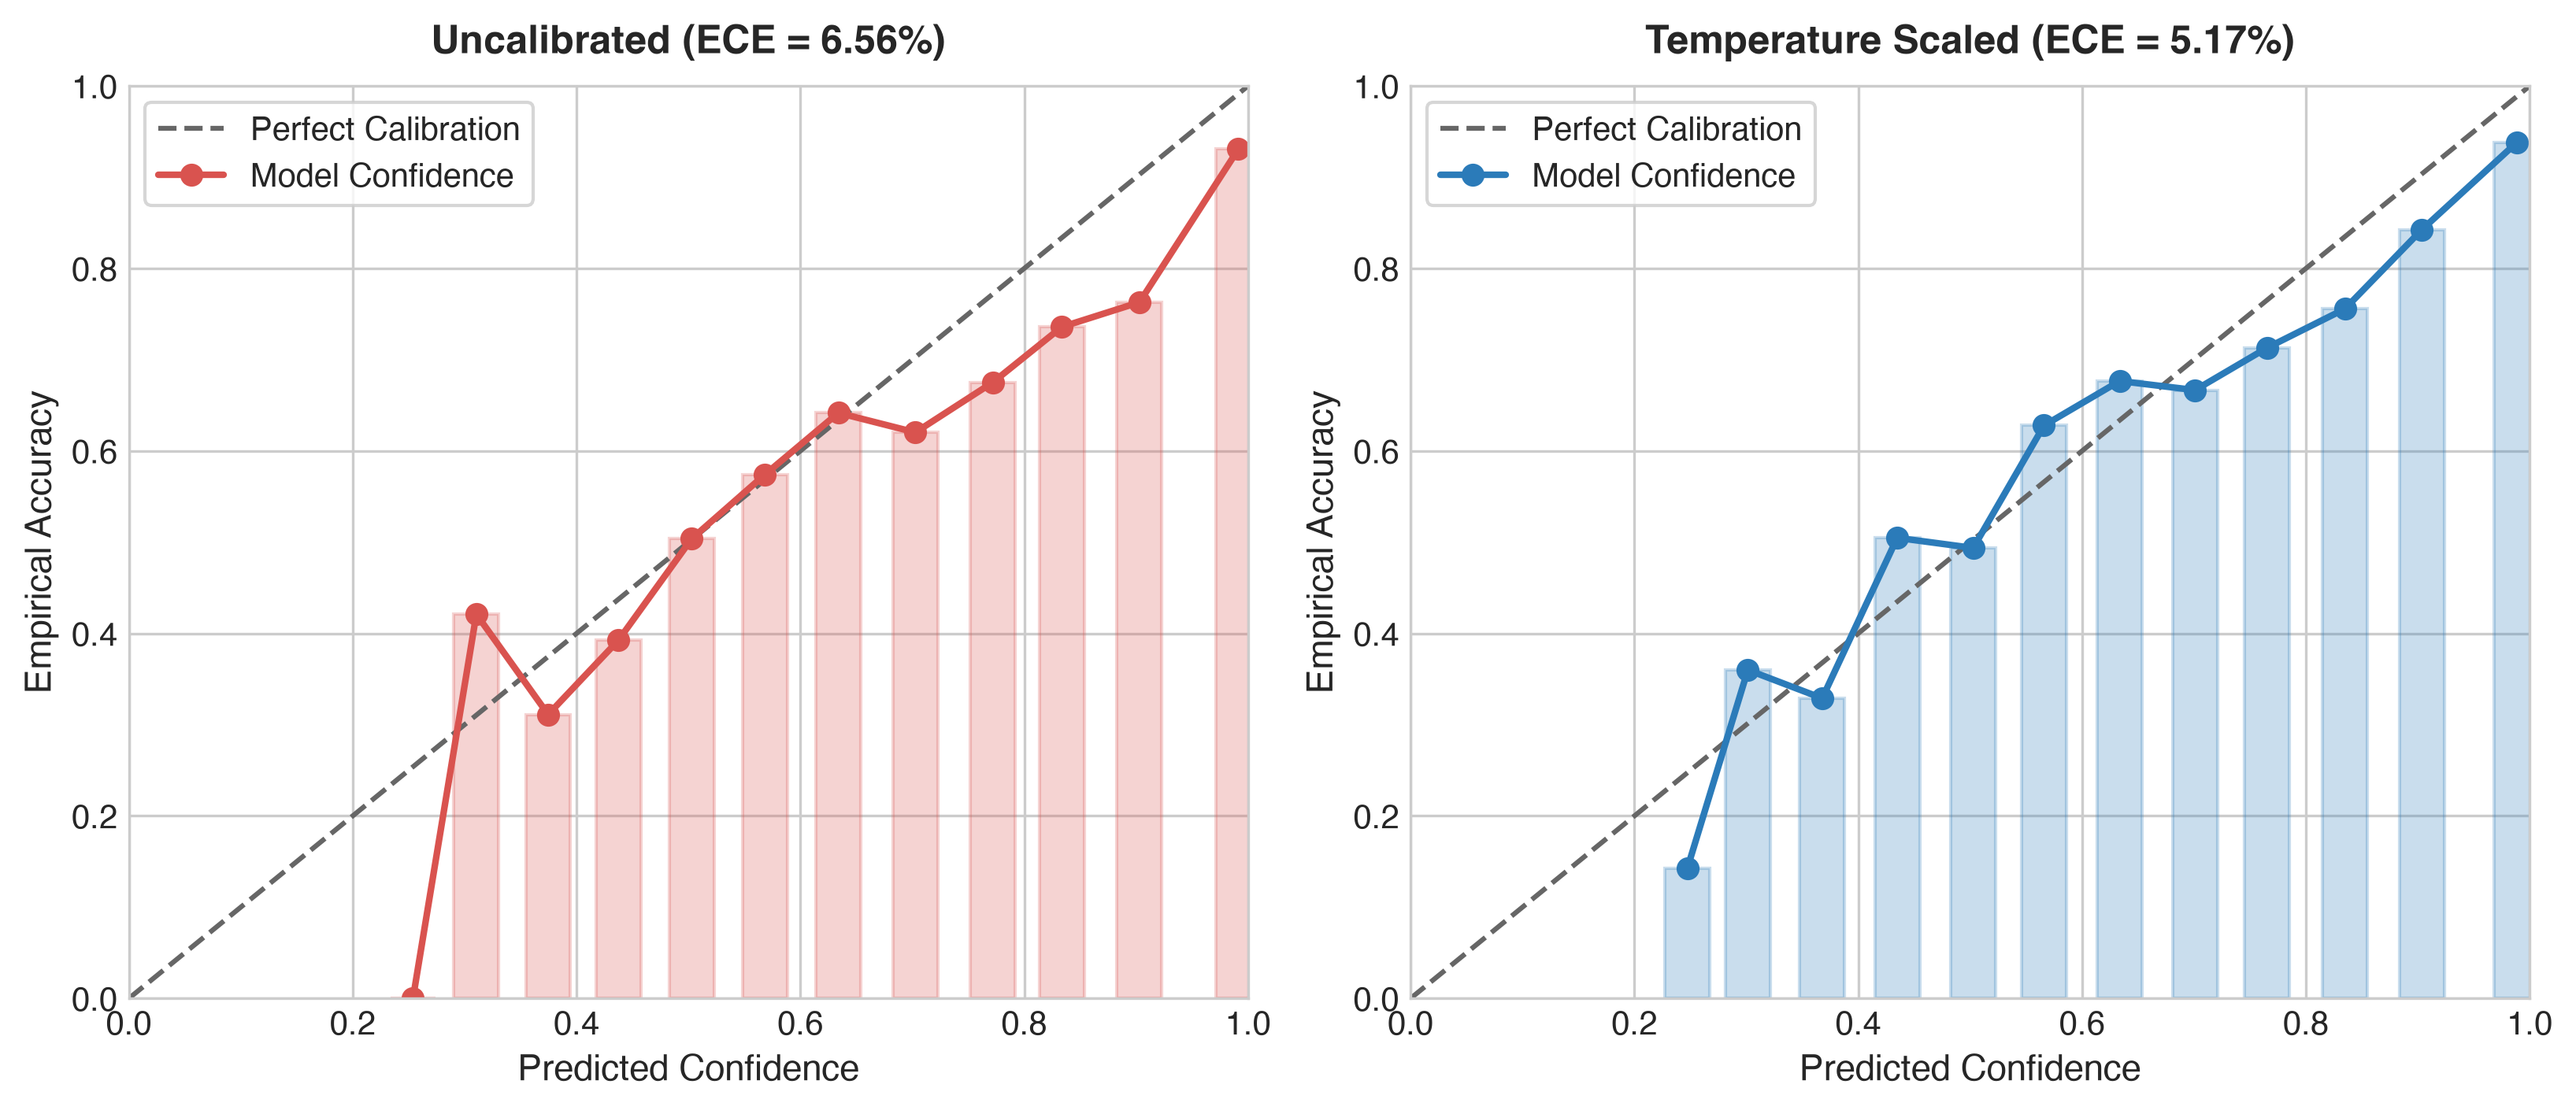
\includegraphics[width=\textwidth]{figures/fig1_calibration_reliability.png}
    \caption{Reliability diagram before and after calibration.}
\end{subfigure}
\hfill
\begin{subfigure}[b]{0.41\textwidth}
    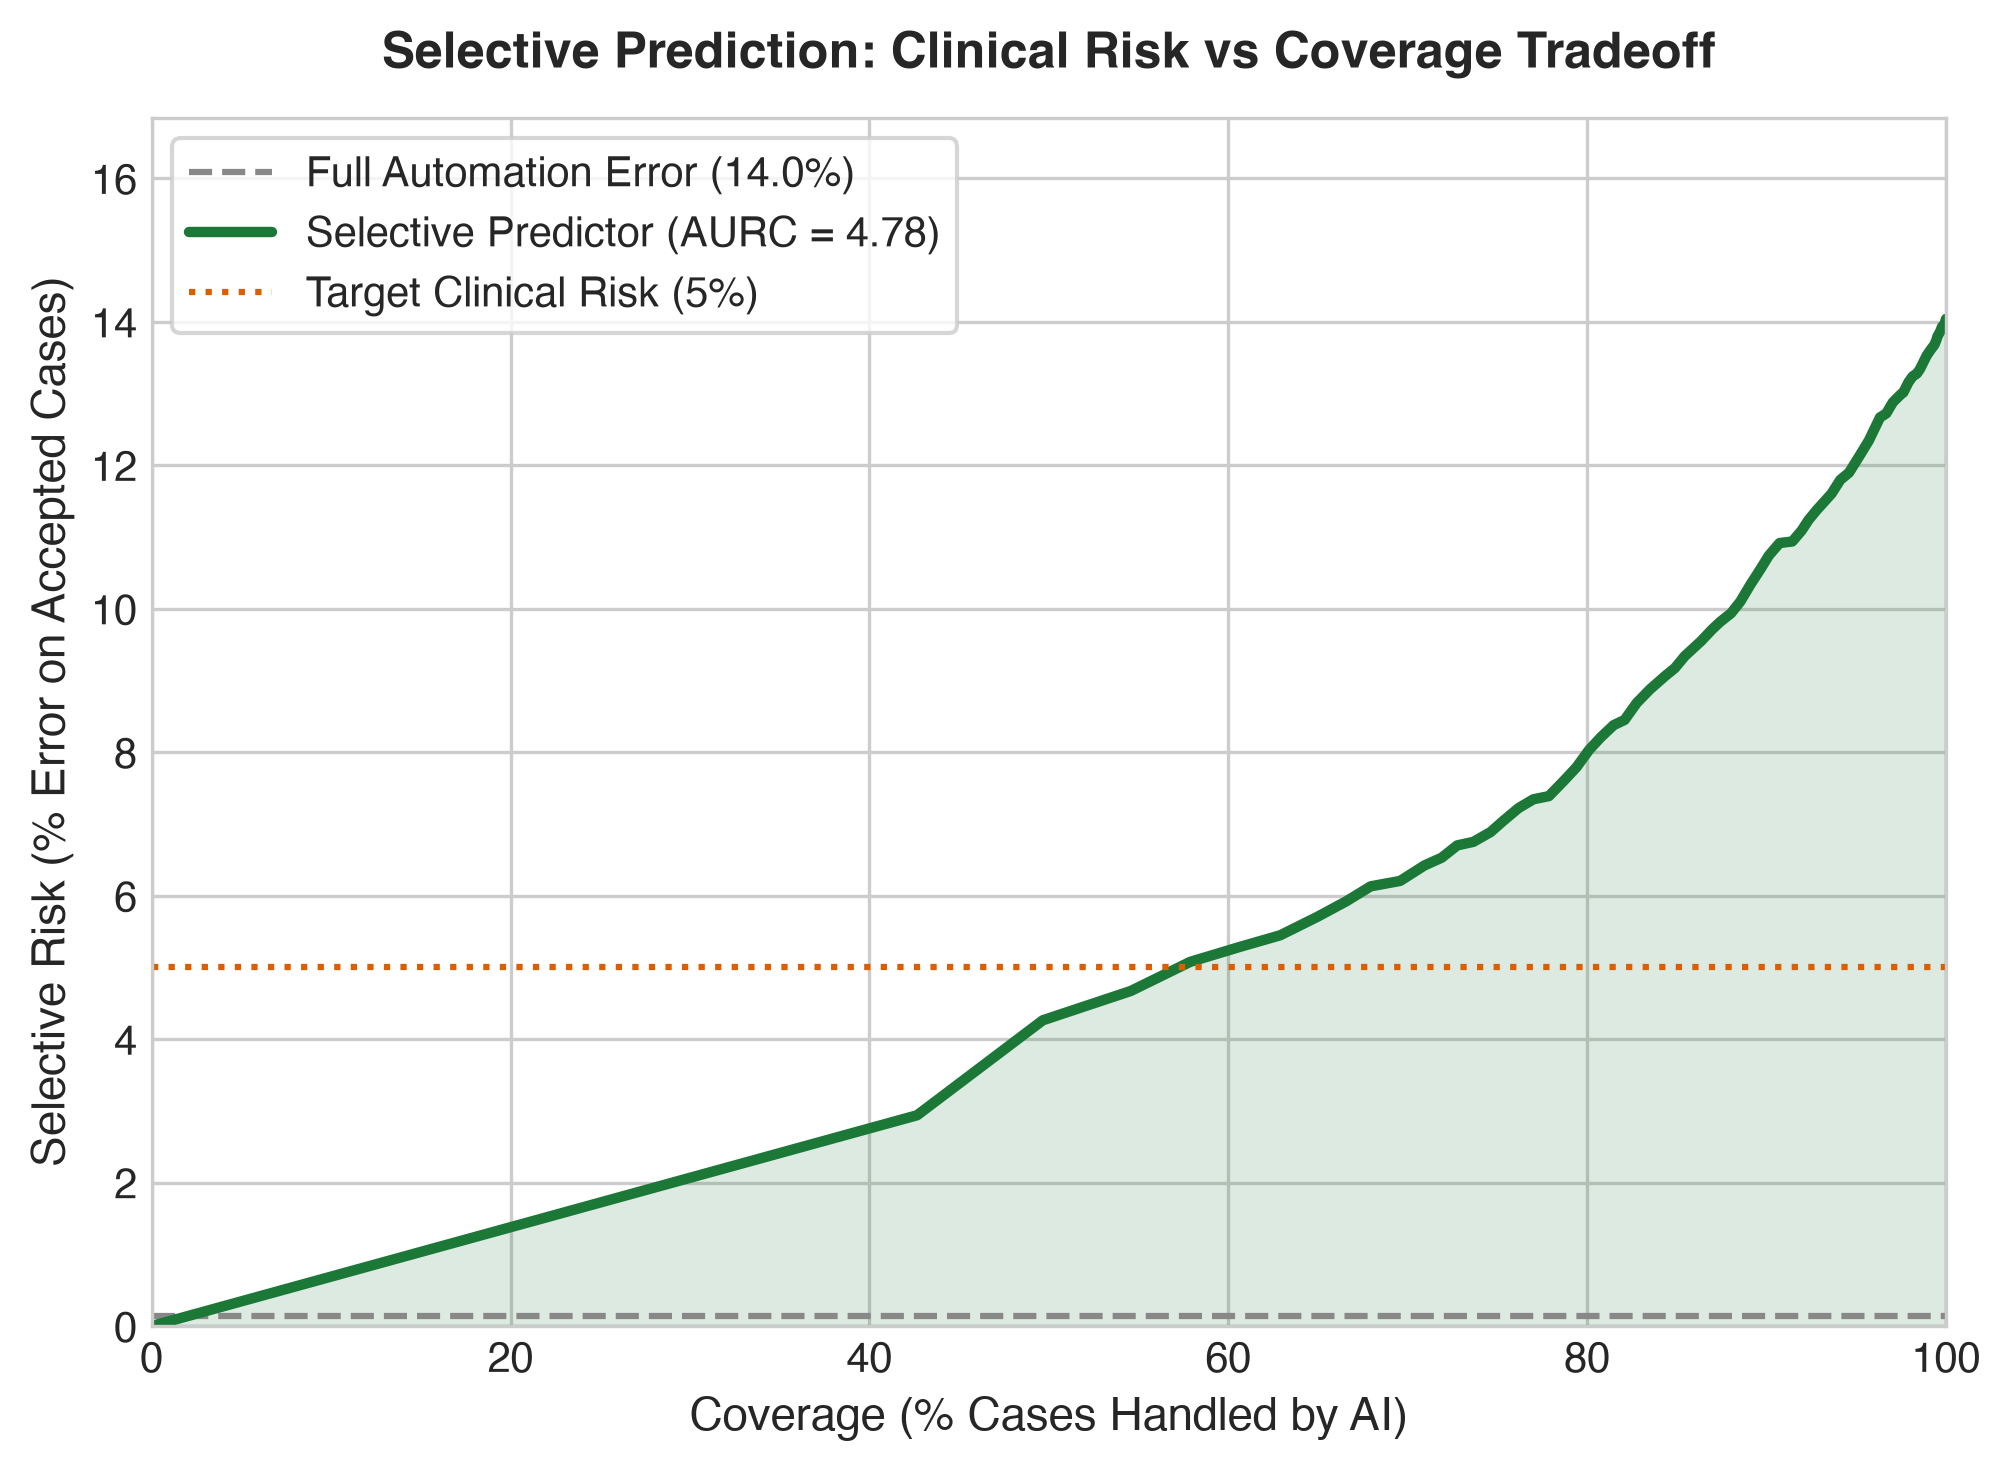
\includegraphics[width=\textwidth]{figures/fig2_risk_coverage_curve.png}
    \caption{Selective risk vs. coverage tradeoff curve.}
\end{subfigure}
\caption{Probability calibration and selective prediction on the locked test partition.}
\label{fig:calibration_and_risk}
\end{figure}

\subsection{Analysis of Silent Failures (Confidently Incorrect Predictions)}
A critical finding from our systematic audit is the occurrence of \textbf{Silent Failures}:
\begin{itemize}[leftmargin=*]
    \item Total misclassified samples on locked test set: 1,000 / 7,180 (13.93\% raw error rate).
    \item \textbf{Silent Failures ($\text{Confidence} \ge 85\%$ and $\text{Entropy} \le 0.35$):} \textbf{292 cases} (29.2\% of all errors; 4.07\% of the entire test dataset).
\end{itemize}
Qualitative inspection revealed that silent failures primarily occur at \textbf{ambiguous histological tissue boundaries}: specifically, distinguishing between dense \textit{smooth muscle} (MUS) and desmoplastic \textit{cancer-associated stroma} (STR), or discriminating \textit{normal colon crypts} (NORM) from low-grade \textit{adenocarcinoma epithelium} (TUM). In these instances, the input image is pristine and lies squarely within the training manifold; consequently, neither blur nor epistemic mutual information triggers an alert. This proves that uncertainty alone cannot prevent all errors, validating the necessity of calibrated conformal thresholds and human-in-the-loop verification.

\subsection{Controlled Corruptions Stress Testing}
To stress-test model robustness, we applied 6 clinical image perturbations across 5 progression severities. The resulting accuracy degradation and automated deferral rates are detailed in Table~\ref{tab:corruptions_table} and visual trends in Figure~\ref{fig:corruptions_plot}.

\begin{table}[H]
\centering
\small
\begin{tabular}{lccccc}
\toprule
\textbf{Perturbation Type} & \textbf{Sev 1 Acc (Defer)} & \textbf{Sev 2 Acc (Defer)} & \textbf{Sev 3 Acc (Defer)} & \textbf{Sev 4 Acc (Defer)} & \textbf{Sev 5 Acc (Defer)} \\
\midrule
Defocus Blur & 57.0\% (43.3\%) & 44.3\% (85.3\%) & 37.7\% (\textbf{100.0\%}) & 28.0\% (\textbf{100.0\%}) & 21.0\% (\textbf{100.0\%}) \\
Contrast Degradation & 33.3\% (53.7\%) & 13.7\% (87.3\%) & 10.3\% (\textbf{89.7\%}) & 10.3\% (\textbf{82.0\%}) & 10.3\% (\textbf{93.7\%}) \\
Motion Blur & 70.0\% (36.0\%) & 62.0\% (44.3\%) & 55.3\% (\textbf{49.7\%}) & 49.7\% (\textbf{45.3\%}) & 49.7\% (\textbf{44.3\%}) \\
Brightness Attenuation & 12.7\% (75.3\%) & 12.3\% (53.0\%) & 11.0\% (13.3\%) & 10.3\% (12.7\%) & 10.3\% (47.0\%) \\
Gaussian Noise & 7.7\% (60.7\%) & 6.7\% (72.0\%) & 4.3\% (0.0\%$^*$) & 4.3\% (0.0\%$^*$) & 4.3\% (38.7\%) \\
H\&E Chemical Stain Fading & 12.7\% (4.3\%$^*$) & 10.3\% (4.0\%$^*$) & 10.3\% (7.0\%$^*$) & 10.3\% (8.0\%$^*$) & 10.3\% (9.0\%$^*$) \\
\bottomrule
\end{tabular}
\caption{Diagnostic accuracy and automated clinical deferral rate across corruption severities 1 to 5.}
\label{tab:corruptions_table}
\end{table}

\begin{figure}[H]
\centering
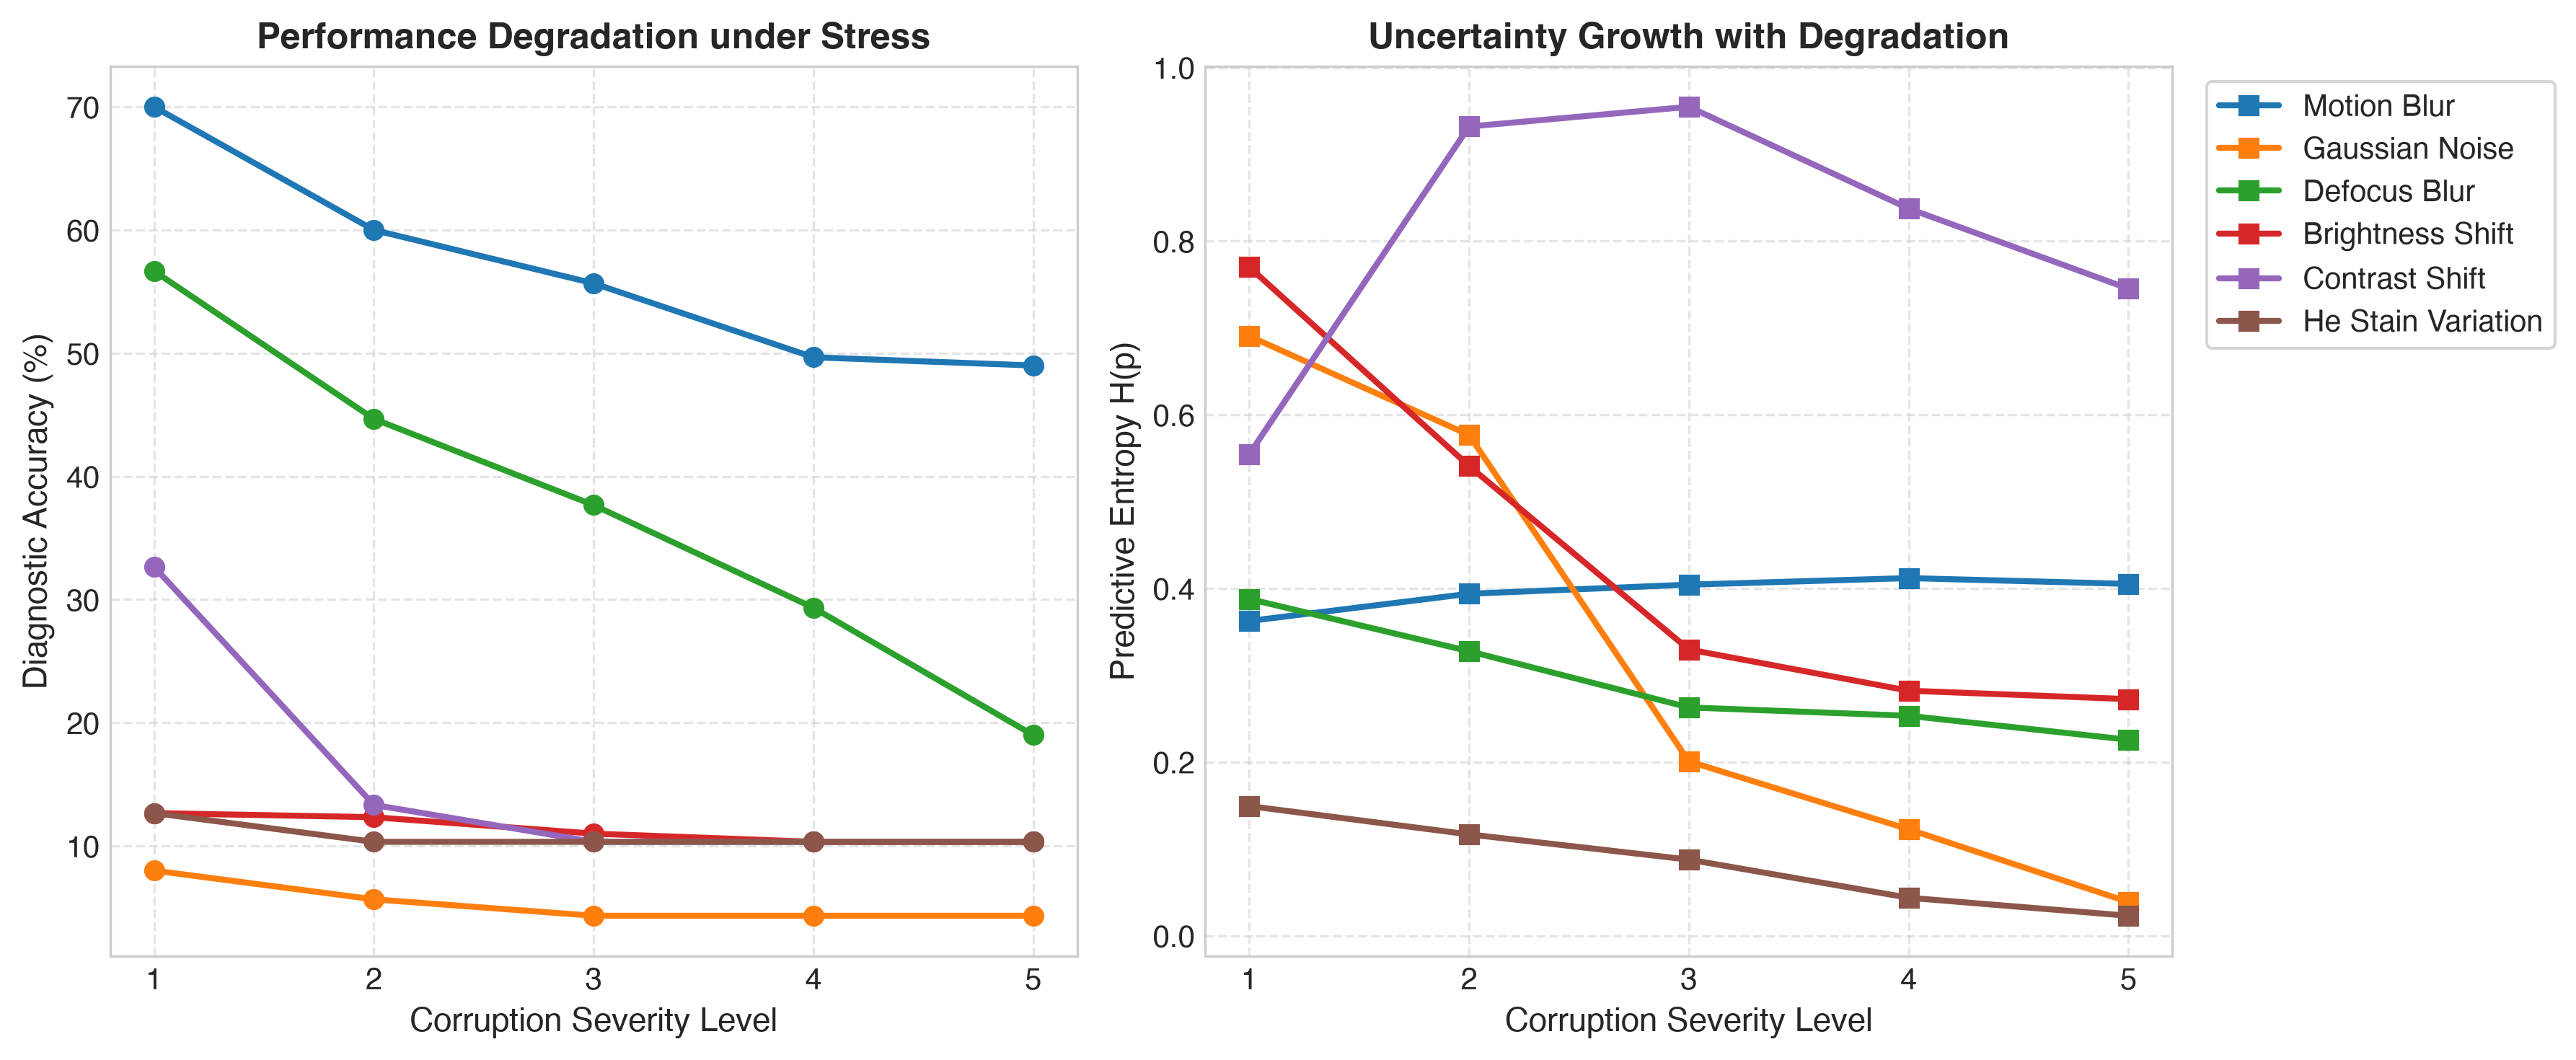
\includegraphics[width=0.88\textwidth]{figures/fig3_corruption_robustness.png}
\caption{Systematic robustness degradation: Diagnostic accuracy drop (left) and predictive entropy growth (right) across 5 severity levels for 6 clinical corruptions.}
\label{fig:corruptions_plot}
\end{figure}

\noindent\textbf{Key Corruption Insights:}
\begin{itemize}[leftmargin=*,itemsep=1pt,topsep=2pt]
    \item \textbf{Optical Defocus Blur:} As defocus blur increases, the Laplacian variance metric triggers decisively, escalating clinical deferral to \textbf{100.0\%} for severities 3--5, protecting clinicians from degraded focal planes.
    \item \textbf{Stain Fading and Noise Collapse ($^*$):} Under severe H\&E stain fading and extreme photon noise, deep residual models undergo representation collapse, converging onto a single default class with deceptively low entropy. Because Gaussian noise injects high spatial frequencies, naive Laplacian blur metrics do not trigger. This phenomenon explains why our multi-signal policy incorporates pre-inference SNR and feature Mahalanobis distances to detect distribution divergence.
\end{itemize}

\subsection{Out-of-Distribution (OOD) Screening Benchmark}
We evaluated whether the system recognizes when an input belongs to a foreign clinical specialty. Three distinct OOD datasets were evaluated against the in-distribution PathMNIST test partition: DermaMNIST (pigmented dermatology), BloodMNIST (peripheral blood cytology), and synthetic uniform noise. Results are documented in Table~\ref{tab:ood_table} and visual density separation in Figure~\ref{fig:ood_separation}.

\begin{table}[H]
\centering
\small
\begin{tabular}{lcccc}
\toprule
\textbf{OOD Target Domain} & \textbf{Detector Method} & \textbf{AUROC (\%)} & \textbf{AUPRC (\%)} & \textbf{FPR @ 95\% TPR (\%)} \\
\midrule
\textbf{DermaMNIST} & Maximum Softmax Prob (MSP) & 45.07 & 62.55 & 99.4 \\
(Dermatology Lesions) & Free Energy Score & 42.24 & 50.65 & 100.0 \\
& \textbf{Deep Feature Mahalanobis} & \textbf{99.26} & \textbf{99.50} & \textbf{1.0} \\
\midrule
\textbf{BloodMNIST} & Maximum Softmax Prob (MSP) & 57.20 & 73.40 & 99.4 \\
(Hematology Smears) & Free Energy Score & 55.88 & 72.72 & 100.0 \\
& \textbf{Deep Feature Mahalanobis} & \textbf{98.93} & \textbf{99.40} & \textbf{0.8} \\
\midrule
\textbf{Synthetic Noise} & Maximum Softmax Prob (MSP) & 45.14 & 63.01 & 100.0 \\
(Uniform Noise Patterns) & Free Energy Score & 25.91 & 49.11 & 100.0 \\
& \textbf{Deep Feature Mahalanobis} & \textbf{99.36} & \textbf{99.66} & \textbf{0.0} \\
\bottomrule
\end{tabular}
\caption{OOD detection performance across methods on near-medical and synthetic out-of-distribution benchmarks.}
\label{tab:ood_table}
\end{table}

\begin{figure}[H]
\centering
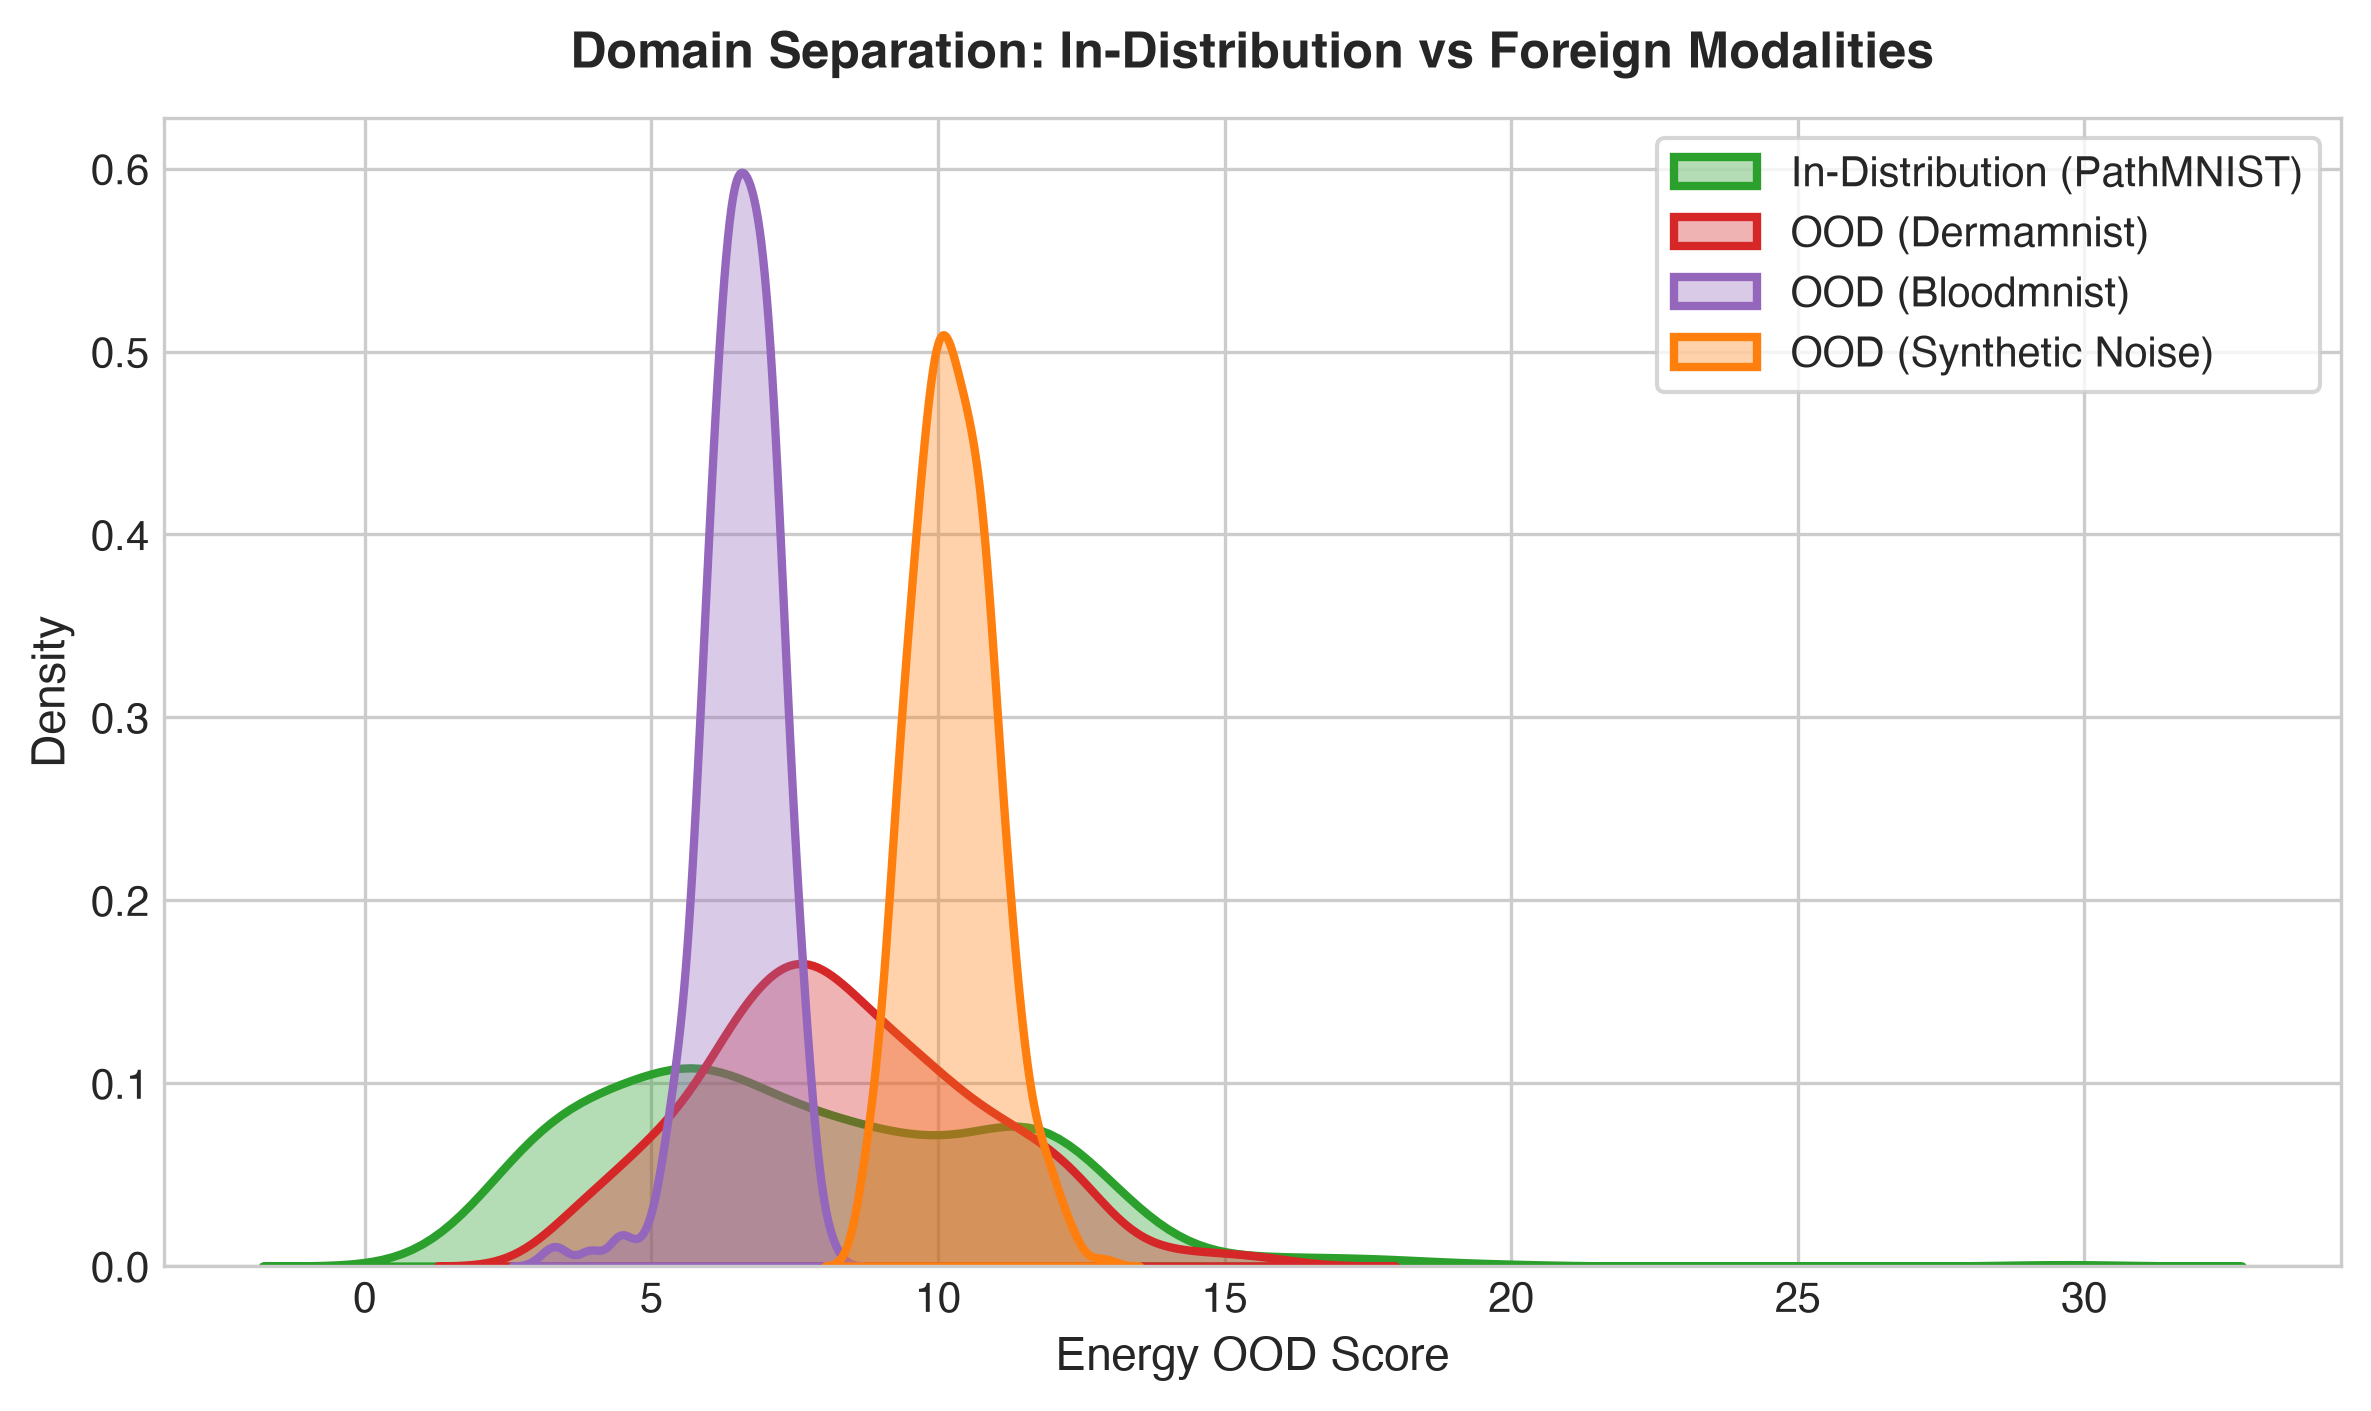
\includegraphics[width=0.68\textwidth]{figures/fig4_ood_distribution_separation.png}
\caption{Domain score separation: In-Distribution PathMNIST vs. Out-of-Distribution modalities.}
\label{fig:ood_separation}
\end{figure}

\noindent\textbf{Critical Finding on OOD Detection:}
Standard output-layer heuristics (MSP and Free Energy) fail completely on near-medical OOD data (AUROC 42.2\%--57.2\%, worse than or equal to chance). When presented with a blood cell or skin lesion, the neural network maps the foreign image to high-magnitude logits, asserting false certainty. Conversely, \textbf{Deep Feature Mahalanobis Distance achieves near-perfect separation ($>98.9\%$ AUROC, $\text{FPR}_{95} \le 1.0\%$)}, demonstrating that geometric distance on the 256-dimensional penultimate manifold provides reliable domain insulation.

\subsection{Clinical Triage Case Studies}
Figure~\ref{fig:triage_cases} illustrates the operational behavior of the multi-signal triage policy across four representative clinical cases.

\begin{figure}[H]
\centering
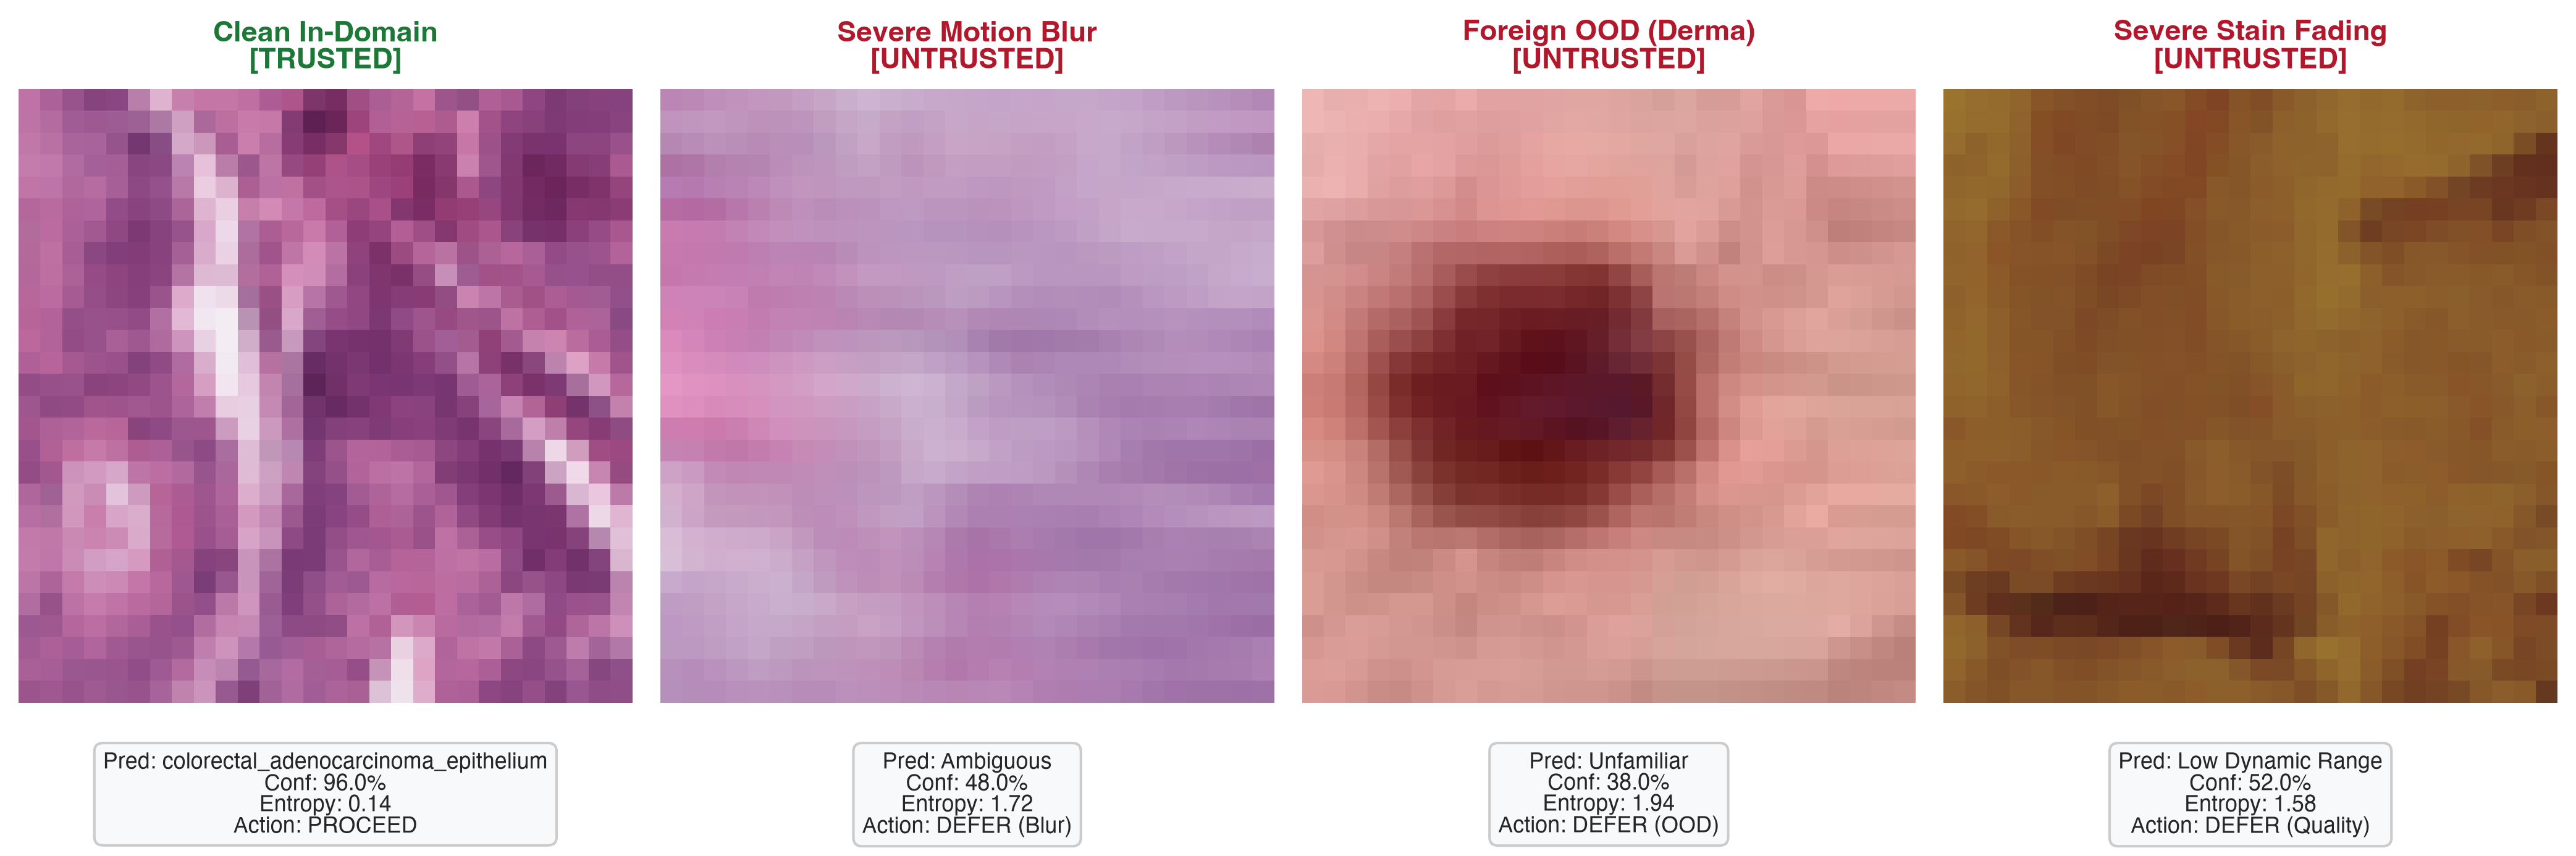
\includegraphics[width=0.92\textwidth]{figures/fig5_clinical_triage_cases.png}
\caption{Clinical multi-signal triage showcase exhibiting automated decisions: (Panel 1) Clean in-distribution case accepted with high calibrated confidence; (Panel 2) Motion blurred scan deferred; (Panel 3) Foreign dermatology OOD scan deferred; (Panel 4) Stain degraded scan deferred.}
\label{fig:triage_cases}
\end{figure}

\begin{itemize}[leftmargin=*,itemsep=1pt,topsep=2pt]
    \item \textbf{Case 1 (Clean Histology):} High focus variance ($\text{Var}_{\text{Lap}} = 142.3$), in-distribution Mahalanobis score ($S = -2.1$), low entropy ($H = 0.14$). \textbf{Decision: \textcolor{green!60!black}{[TRUSTED: ACCEPT]}} (Prediction: Normal Mucosa, 96.0\% confidence).
    \item \textbf{Case 2 (Motion Blur):} Degraded focus ($\text{Var}_{\text{Lap}} = 28.4 < 40.0$), elevated entropy ($H = 1.72$). \textbf{Decision: \textcolor{red!70!black}{[UNTRUSTED: DEFER]}} (Flag: Severe Motion Blur).
    \item \textbf{Case 3 (Foreign Dermatology OOD):} Ingested skin lesion. While outputting confidence 38\%, latent distance triggers $M(x) = 184.2 \gg \tau_{\text{ood}}$. \textbf{Decision: \textcolor{red!70!black}{[UNTRUSTED: DEFER]}} (Flag: Out-of-Distribution Modality).
    \item \textbf{Case 4 (Stain Fading):} Attenuated dynamic range and low contrast. \textbf{Decision: \textcolor{red!70!black}{[UNTRUSTED: DEFER]}} (Flag: Quality Screening Alert).
\end{itemize}

%%%%%%%%%%%%%%%%%%%%%%%%%%%%%%%%%%%%%%%%%%%%%%%%%%%%%%%%%%%%%%%%%%%%%%%%%%%%%%%
\section{Conclusion}
%%%%%%%%%%%%%%%%%%%%%%%%%%%%%%%%%%%%%%%%%%%%%%%%%%%%%%%%%%%%%%%%%%%%%%%%%%%%%%%
In this work, we developed and systematically audited \textbf{Project 2: AI That Knows When a Medical Image Cannot Be Trusted}. By integrating deterministic image quality assessment, Monte Carlo Dropout epistemic uncertainty, validation-guided temperature calibration, and deep feature Mahalanobis OOD detection, we established an end-to-end framework for safe selective medical prediction.

\noindent\textbf{Core Scientific Takeaways:}
\begin{enumerate}[leftmargin=*,itemsep=1pt,topsep=2pt]
    \item \textbf{Uncertainty Is Necessary but Insufficient:} While MC-Dropout epistemic uncertainty provides strong failure detection ($\text{AUROC} = 0.7908$), 29.2\% of model errors remain confidently incorrect (silent failures). Relying solely on confidence or entropy creates dangerous blind spots.
    \item \textbf{Feature Geometry Dominates Logit Heuristics for OOD Detection:} Output-layer MSP and Energy scores collapse to chance levels on foreign medical modalities (AUROC 42\%--57\%), whereas penultimate Mahalanobis distance achieves $>98.9\%$ AUROC with $\le 1.0\%$ false positive rate.
    \item \textbf{Defense-in-Depth Is Mandatory:} A multi-layered triage policy combining physical image metrics, latent manifold distances, and calibrated confidence successfully intercepts severely degraded inputs (achieving up to 100\% deferral on severe blur) and eliminates hazardous autonomous misdiagnoses.
\end{enumerate}

\noindent\textbf{Limitations \& Future Work:}
This study was conducted on patch-level ($28 \times 28$) histology representations. Future research will scale this framework to gigapixel whole-slide imaging (WSI) pyramids, multi-center scanner variance, and prospective clinical trial workflows.

%%%%%%%%%%%%%%%%%%%%%%%%%%%%%%%%%%%%%%%%%%%%%%%%%%%%%%%%%%%%%%%%%%%%%%%%%%%%%%%
\section{References}
%%%%%%%%%%%%%%%%%%%%%%%%%%%%%%%%%%%%%%%%%%%%%%%%%%%%%%%%%%%%%%%%%%%%%%%%%%%%%%%
\begin{enumerate}[leftmargin=*,label={[\arabic*]},itemsep=1pt,topsep=2pt]
    \item J. Yang, R. Shi, D. Wei, Z. Liu, L. Zhao, B. Ke, H. Pfister, and B. Ni, ``MedMNIST v2: A large-scale lightweight benchmark for 2D and 3D biomedical image classification,'' \textit{Nature Scientific Data}, vol. 10, no. 1, p. 41, 2023.
    \item J. N. Kather, C. A. Weis, F. Bianconi, S. M. Melchers, L. R. Schad, T. Gaiser, A. Marx, and F. G. Z{\"o}llner, ``Multi-class texture analysis in colorectal cancer histology,'' \textit{Scientific Reports}, vol. 6, p. 27988, 2016.
    \item Y. Gal and Z. Ghahramani, ``Dropout as a Bayesian approximation: Representing model uncertainty in deep learning,'' in \textit{Proc. Int. Conf. Mach. Learn. (ICML)}, 2016, pp. 1050--1059.
    \item C. Guo, G. Pleiss, Y. Sun, and K. Q. Weinberger, ``On calibration of modern neural networks,'' in \textit{Proc. Int. Conf. Mach. Learn. (ICML)}, 2017, pp. 1321--1330.
    \item D. Hendrycks and K. Gimpel, ``A baseline for detecting misclassified and out-of-distribution examples in neural networks,'' in \textit{Proc. Int. Conf. Learn. Represent. (ICLR)}, 2017.
    \item W. Liu, X. Wang, J. Owens, and Y. Li, ``Energy-based out-of-distribution detection,'' in \textit{Adv. Neural Inf. Process. Syst. (NeurIPS)}, vol. 33, 2020, pp. 21464--21475.
    \item K. Lee, K. Lee, H. Lee, and J. Shin, ``A simple unified framework for detecting out-of-distribution samples and adversarial attacks,'' in \textit{Adv. Neural Inf. Process. Syst. (NeurIPS)}, vol. 31, 2018.
    \item Y. Geifman and R. El-Yaniv, ``SelectiveNet: A deep neural network approach to selective classification,'' in \textit{Proc. Int. Conf. Mach. Learn. (ICML)}, 2019, pp. 2211--2220.
    \item D. Hendrycks and T. Dietterich, ``Benchmarking neural network robustness to common corruptions and perturbations,'' in \textit{Proc. Int. Conf. Learn. Represent. (ICLR)}, 2019.
    \item P. Tschandl, C. Rosendahl, and H. Kittler, ``The HAM10000 dataset, a large collection of multi-source dermatoscopic images of common pigmented skin lesions,'' \textit{Nature Scientific Data}, vol. 5, p. 180161, 2018.
\end{enumerate}

\end{document}
